\documentclass[12pt, class=report, crop=false]{standalone}
\usepackage{ba_thesis}

\begin{document}

% \addcontentsline{toc}{chapter}{Introduction}
\chapter{Electromagnetism and Laser Profiles}%
\label{chap:electromagnetism}

\section{Classical Electrodynamics}

The main principles and laws that govern the phenomena behind lasers, plasma and their interaction are those of classical electrodynamics. As such, like many others tackling this area of research, I find that adding an overview of electrodynamics is simply mandatory. My aim when it comes to differentiating this introductory review from the millions of others out there, if at all possible, is to offer thorough calculations and explanations on some aspects where I personally felt like I wanted to see things from a clearer perspective.

\subsection{Maxwell's Equations}

The Maxwell equations are~(\cite{jacksonClassicalElectrodynamics1999}):

\begin{subequations}
  \label{eq:maxwell-general}
  \begin{align}
    \div{\vb{D}} & = \rho
    \label{eq:coulomb-law-general} \\
    \div{\vb{B}} & = 0
    \label{eq:gauss-law-general} \\
    \curl{\vb{E}} & = - \pdv{\vb{B}}{t}
    \label{eq:faraday-law-general} \\
    \curl{\vb{H}} & = \vb{j} + \pdv{\vb{D}}{t}
    \label{eq:ampere-law-general} \,.
  \end{align}
\end{subequations}

In the absence of magnetic and polarizable media, \(\vb{D}=\varepsilon_0 \vb{E}\) and \(\vb{B}=\mu_0 \vb{H}\) and the equations become:

\begin{subequations}
  \label{eq:maxwell}
  \begin{align}
    \div{\vb{E}} & = \frac{\rho}{\varepsilon_0} \label{eq:coulomb-law} \\
    \div{\vb{B}} & = 0 \label{eq:gauss-law} \\
    \curl{\vb{E}} & = - \pdv{\vb{B}}{t} \label{eq:faraday-law} \\
    \curl{\vb{B}} & = \mu_0 \vb{j} + \frac{1}{c^2} \pdv{\vb{E}}{t} \,, \label{eq:ampere-law}
  \end{align}
\end{subequations}

\par
While most readers probably have already had at least a basic introduction to the phenomena from which these equations arise and are well acquainted to how to make use of these equations, I would direct those who haven't towards the book by~\cite{fleischStudentGuideMaxwell2008}%

\par
By extracting the current density from~\cref{eq:ampere-law}, computing its divergence and then replacing the electric field term using~\cref{eq:coulomb-law} one obtains the continuity equation, which relates only the field sources to one another:

\begin{equation}
  \label{eq:continuity-equation}
  \div{\vb{j}(\vb{r}, t)} + \pdv{\rho(\vb{r}, t)}{t} = 0 \,.
\end{equation}

\par
These equations are also complemented by the Lorentz force, which describes how the fields act on the sources. The expression of the Lorentz force in the contiuous case is:

\[
  \vb{F} = \int_\mathcal{V} \dd{\vb{r}'} \left[ \rho(\vb{r}', t) \vb{E}(\vb{r}', t) +
           \frac{1}{c} \vb{j}(\vb{r}', t) \cross \vb{B}(\vb{r}', t)\right] .
\]

\subsection{The Scalar and Vector Potentials}

Since the electric~(\(\vb{E}\)) and magnetic~(\(\vb{B}\)) fields are vectors, they can be described together by a total of six quantities. The sources on the other hand can be described using only four quantities: the electric charge density~\(\rho\) and the three components of the electric current density~\(\vb{j}\). This points to the fact that there is a more convenient way to describe the fields. In finding this alternative, we shall employ the following basic results from algebra:
\begin{subequations}
  \label{id:algebra}
  \begin{align}
    \div{(\curl{\vb{v}})}=0
    \label{id:div-rot} \\
    \curl{(\div{\vb{v}})}=0
    \label{id:rot-div} \\
    \curl{(\grad{f})}=0
    \label{id:rot-grad} \,,
  \end{align}
\end{subequations}
which are valid for any vector function~\(\vb{v}\) and for any scalar function~\(f\).

\par
From~\cref{eq:gauss-law,id:div-rot} one can define the vector potential \(\vb{A}\) such that

\begin{equation}
  \label{eq:vector-potential}
  \vb{B}(\vb{r}, t) = \curl{\vb{A}(\vb{r}, t)}\,.
\end{equation}
By substituting~\eqref{eq:vector-potential} in~\eqref{eq:faraday-law} one obtains

\begin{equation}
  \label{eq:faraday-vector-potential}
  \curl(\vb{E} + \pdv{\vb{A}}{t}) = 0
\end{equation}
which together with~\cref{id:rot-grad} defines the scalar potential \(\phi\)

\begin{equation}
  \label{eq:faraday-scalar-potential}
  \grad{\phi}(\vb{r}, t) = -\vb{E}(\vb{r}, t) - \pdv{\vb{A}}{t}\,.
\end{equation}
Using this in~\cref{eq:coulomb-law}

\begin{equation}
  \label{eq:coulomb-scalar-potential}
  \laplacian{\phi} + \pdv{t}\div{\vb{A}} = - \frac{\rho}{\varepsilon_0}\,.
\end{equation}
Similarly, using~\cref{eq:faraday-scalar-potential} in~\cref{eq:ampere-law} and making use of the following vector identity

\begin{equation}
  \label{eq:curl-of-curl}
  \curl(\curl{\vb{v}}) = \grad(\div{\vb{v}}) - \laplacian{\vb{v}}\,,
\end{equation}
another equation of the potentials is obtained

\begin{equation}
  \label{eq:ampere-potentials}
  \laplacian{\vb{A}} - \frac{1}{c^2}\pdv[2]{\vb{A}}{t} =
    -\mu_0 \vb{j} + \grad(\div{\vb{A}} + \frac{1}{c^2} \pdv{\phi}{t})\,.
\end{equation}

Considering that at every step in the derivation of~\cref{eq:coulomb-scalar-potential,eq:ampere-potentials} we only imposed the Maxwell equations and basic algebraic identities, it follows that~\cref{eq:coulomb-scalar-potential,eq:ampere-potentials} and~\cref{eq:maxwell} are completely equivalent.
We now have reduced the six quantities describing the fields to only four: the scalar potential~\(\phi\) and the three components of the vector potential~\(\vb{A}\).
This description of the fields through the potentials is quite useful since it is easily integrated in the formalism of special relativity. One can define the electomagnetic potential 4-vector such that the scalar field is the time-like component and the vector field is the space-like component.

In general, when studying the dynamics of particles in an electomagnetic field, once the potentials are computed using~\cref{eq:coulomb-scalar-potential,eq:ampere-potentials} the fields are obtained from~\cref{eq:vector-potential,eq:faraday-scalar-potential} and can be used further in the expression of the Lorentz force.

\subsection{Gauge Transformation}
\label{ch-ref-1}
By a direct application of~\cref{id:algebra} one can show that a simultaneous transformation by an arbitrary well-behaved (continuous with continuous derivatives) scalar function~\(f=f(\vb{r},t)\) of the potentials:

\begin{subequations}
  \label{gauge}
  \begin{align}
    \phi \rightarrow \phi + \pdv{f}{t} \\
    \vb{A} \rightarrow \vb{A} - \grad{f} \,,
  \end{align}
\end{subequations}
leaves the electric and magnetic field unchanged. This is actually a quite natural equivalent of the intuitive fact that any potential is defined up to a constant. In the particular case of the electromagnetic potential,~\cref{gauge} define a gauge transformation. There are two widely used gauges.

\paragraph{Lorenz gauge}

\begin{equation}
  \label{eq:lorenz-gauge}
  \div{\vb{A}} + \frac{1}{c^2} \pdv{\phi}{t}=0
\end{equation}

\par
This gauge cancels the gradient in~\cref{eq:ampere-potentials}. If one works in the usual Mikovski metric~(\cite{weinbergGravitationCosmologyPrinciples1972})

\begin{equation}
  \label{metric}
  \eta_{\mu \nu} =
    \begin{pmatrix}
      -1 & 0 & 0 & 0 \\
      0 & 1 & 0 & 0 \\
      0 & 0 & 1 & 0 \\
      0 & 0 & 0 & 1
    \end{pmatrix}
\end{equation}

the d'Alembert operator is then defined as
\[
\Box = \partial^{\mu} \partial_{\mu} = \eta^{\mu \nu} \partial_{\nu} \partial_{\mu} = \laplacian{} - \frac{1}{c^{2}} \pdv[2]{}{t} \,,
\]
where \(\mu,\,\nu=\overline{0,3}\) with 0 being the temporal index and 1, 2, 3 being the spatial indices (note: in this thesis I use Einstein's summation convention whenever there is and index repeated once up and down, \(\textit{i}.\textit{e}.\) is appears as both variant and covariant in a product). By replacing this definition in~\cref{eq:coulomb-scalar-potential,eq:ampere-potentials}, it is easy to see that both \(\vb{A}\) and \(\phi\) obey a free wave equation:

\begin{subequations}
  \begin{align}
    \Box \vb{A} = -\mu_0 \vb{j}\\
    \Box \phi = -\frac{\rho}{\varepsilon_0}  \,.
  \end{align}
\end{subequations}

\paragraph{Coulomb Gauge (sometimes found as transversal/velocity gauge)}

\begin{equation}
  \div{\vb{A}} = 0
\end{equation}

\par
Under this gauge, the potential equations~\cref{eq:coulomb-scalar-potential,eq:ampere-potentials} take the form:

\begin{subequations}
  \begin{align}
    \Box \vb{A} = -\mu_0 \vb{j} + \frac{1}{c^{2}} \grad{\pdv{\phi}{t}}\\
    \laplacian{\phi} = -\frac{\rho}{\varepsilon_0}  \,.
  \end{align}
\end{subequations}

\subsection{The Poynting Theorem}
\label{section:poynting}
The Poynting theorem is the form of the conservation of energy in the case of electromagnetic fields interacting with charges and currents. Since it is such an important and general result, this presentation of it will start from the more general form of the Maxwell equations~\cref{eq:maxwell-general}.
\par
In the derivation of this theorem, one usually starts from the local form of the Lorentz force~(\cite{griffithsIntroductionElectrodynamics1999}):

\begin{equation*}
  \vb{F} = \delta q \vb{E} + \delta q \vb{v} \cp \vb{B}
\end{equation*}

\par

The work done by the electric field part of the force on the volume element with charge \( \delta q \) and velocity \( \vb{v} = \dv{\vb{l}}{t} \) is

\begin{equation*}
  \dd{W_{e}} = q \dd{\vb{l}} \vdot \vb{E}
\end{equation*}
and the corresponding rate of work done is

\begin{equation*}
  \dv{W_{e}}{t} = q \vb{v} \vdot \vb{E}
\end{equation*}
while for the magnetic part we have (as expected)

\begin{equation*}
  \dd{W_{m}} = \dd{\vb{l}} \vdot \vb{F_{b}} = q \dd{\vb{l}} \vdot ( \vb{v} \cp \vb{B})
\end{equation*}

\begin{equation*}
  \dv{W_{b}}{t} = q \vb{v} \vdot ( \vb{v} \cp \vb{B}) = 0 \,.
\end{equation*}

\par
Adding these contributions and generalizing for the case of a distribution of charges and currents one obtains

\begin{equation}
  \dv{W}{t} = \int_\mathcal{V} \dd{\vb{r}} \vb{E}\vdot\vb{j}
\end{equation}

By extracting \(\vb{j}\) from~\cref{eq:ampere-law-general} and replacing in the above equation we have

\begin{equation*}
  \dv{W}{t} = \int_\mathcal{V} \dd{\vb{r}} \left[ \vb{E}\vdot (\curl{\vb{H}}) - \vb{E}\vdot \pdv{\vb{D}}{t} \right]
\end{equation*}
Employing here the vector identity here

\begin{equation}
  \label{id:grad-of-vector-product}
  \grad{(\vb{u}\cp\vb{v})} = \vb{v}\vdot(\curl{\vb{u}})-\vb{u}\vdot(\curl{\vb{v}})
\end{equation}
gives

\begin{equation*}
  \dv{W}{t} = \int_\mathcal{V} \dd{\vb{r}} \left[ \vb{H}\vdot (\curl{\vb{E}}) - \grad{(\vb{E}\cp\vb{H})} - \vb{E}\vdot \pdv{\vb{D}}{t} \right] \,.
\end{equation*}
Replacing the curl of \( \vb{E}\) using Faraday's law~(\ref{eq:faraday-law-general}) we finally obtain

\begin{equation*}
  \dv{W}{t} = - \int_\mathcal{V} \dd{\vb{r}} \left[ \grad{(\vb{E}\cp\vb{H})} + \vb{E}\vdot \pdv{\vb{D}}{t} + \vb{H}\vdot \pdv{\vb{B}}{t} \right] \,.
\end{equation*}

If we restric the discussion now only to linar media (\textit{i}.\textit{e}. \(\vb{D}=\varepsilon \vb{E}\) and \(\vb{B} = \mu \vb{H}\)) a new important quantity can be defined

\begin{equation}
  \label{def:energy-density}
  w_{em} = \frac{1}{2} (\vb{E}\vdot\vb{D}+\vb{H}\vdot\vb{B})
\end{equation}
which leads to a new way to write the expression of the rate of work done by the electromagnetic field

\begin{equation}
  \label{th:poynting-0}
  \dv{W}{t} = - \int_\mathcal{V} \dd{\vb{r}} \left[\grad{(\vb{E}\cp\vb{H})} + \pdv{w_{em}}{t}\right] \,,
\end{equation}
where the Poynting vector is

\begin{equation}
  \label{def:poynting-vector}
  \vb{S}=\vb{E}\cp\vb{H}\,.
\end{equation}

In order to complete the derivation of Poynting's theorem, an we must see how it is to be interpreted. As such, a short paranthesis concerning \( w_{em}\) is in order.

\subsubsection{Electrostatic field energy density}
For a system of N stationary point-like charged particles of charges \(q_{i}\) placed at \(\vb{r_{i}} \,,\,i=\overline{1,N}\) in a medium with permittivity \(\varepsilon\), the total potential energy of the system, when neglecting the infinite self-interaction terms, is~(\cite{jacksonClassicalElectrodynamics1999})

\begin{equation*}
  W_{e} = \frac{1}{2} \sum_{i,j=1, i\neq j}^{N} \frac{q_{i} q_{j}}{4 \pi \varepsilon \abs{\vb{r_{i}}-\vb{r_{j}}}}
\end{equation*}
or, factoring out the scalar potential \(\phi (\vb{r_{i}})\) generated by all the other particles at the position of particle i,

\begin{equation*}
  W_{e} = \frac{1}{2} \sum_{i=1}^{N} q_{i} \phi (\vb{r_{i}})
\end{equation*}
This is easily generalized in integral form

\begin{equation*}
  W_{e} = \frac{1}{2} \int_\mathcal{V} \dd{\vb{r}} \rho (\vb{r}) \phi (\vb{r}) \, ,
\end{equation*}
where we use the delta-Dirac function for pointlike particles if needed.

\par
Using the fact that the electrostatic potential is defined by \(\vb{E} = - \grad{\phi}\) and replacing this in~\cref{eq:coulomb-law-general} one obtains the poison equation

\begin{equation}
 \label{eq:poisson}
 \laplacian{\phi} = - \frac{\rho}{\varepsilon} \,.
\end{equation}
With this, the integral above becomes

\begin{equation*}
  W_{e} = \frac{\varepsilon}{2} \int_\mathcal{V} \dd{\vb{r}} \phi \laplacian{\phi} = - \frac{\varepsilon}{2} \int_\mathcal{V} \dd{\vb{r}} \phi \grad{\phi} + \frac{\varepsilon}{2} \int_\mathcal{V} \dd{\vb{r}} \abs{\grad{\phi}}^{2} \, ,
\end{equation*}
where integration by parts has been used.

\par
In order to reach the desired result, we still have to perform one more integration by parts

\begin{equation*}
  \int_\mathcal{V} \dd{\vb{r}} \phi \grad{\phi} = \frac{1}{2} \int_\mathcal{V} \dd{\vb{r}} \grad{\phi^2} = \int_{\mathcal{S}_{\mathcal{V}}} \dd{\vb{a}} \phi^{2} \, ,
\end{equation*}
where in the last step we used Gauss' theorem. Now, if we itegrate over the entire space and keep in mind that the electrostatic potential should be zero at infinity, the above integral becames null. Using again the realtion between the gradient of the potential and the electric field we get

\begin{equation}
  W_{e} = \frac{\varepsilon}{2} \int_\mathcal{V} \dd{\vb{r}} \vb{E}^{2}
\end{equation}
or, equivalently,

\begin{equation}
  W_{e} = \frac{1}{2} \int_\mathcal{V} \dd{\vb{r}} \vb{E} \vdot \vb{D} \,.
\end{equation}

\par
This leads to the definition of the energy density of the electrostatic field

\begin{equation}
  \label{def:electrostatic-en-density}
  w_{e} = \frac{1}{2} \vb{E} \vdot \vb{D} \,.
\end{equation}

\subsubsection{Magnetostatic field energy density}

This time around we start with a current loop in the case of magnetostatics (\(\div{\vb{j}}=0\)). No matter the current distribution in space, since the current density is rotational, we can always divide it in individual infinitesimal current loops. A change in the magnetic flux through such a loop is given by the integral form of Faraday's law~(\ref{eq:faraday-law-general})

\begin{equation}
  e = \oint_{\gamma} \dd{\vb{l}}\vdot\vb{E} = - \dv{\phi_{B}}{t} \,,
\end{equation}
where \(\gamma\) is the closed curve describing the loop and \(\phi_{B}\) is the magnetic flux through the loop.

\par
Since the autoinduced magnetic flux is \(\phi_{B}=LI\), where \(L\) is the inductance of the loop and \(I\) the intensity of the electric current flowing in it, the electromotive force caused by autoinduction is

\begin{equation*}
  e = -L \dv{I}{t} \,.
\end{equation*}
Thus the rate of work against the increase of the current is

\begin{equation*}
  \dv{W_{B}}{t} = - I e = LI \dv{I}{t} = \dv{t} (\frac{LI^{2}}{2})\,.
\end{equation*}
With this result we obtain the energy necessary to get a current of intensity \(I\) starting through a loop:

\begin{equation*}
  W_{B} = \frac{LI^2}{2} \,.
\end{equation*}

\par
We will now eliminate \(L\) the same way we introduced it

\begin{equation*}
  \phi_{B} = LI = \int_{\mathcal{S}_\mathcal{\gamma}} \dd{\vb{a}} \vdot \vb{B} =  \int_{\mathcal{S}_\mathcal{\gamma}} \dd{\vb{a}} \vdot (\curl{\vb{A}}) = \oint_{\gamma} \dd{\vb{l}}\vdot \vb{A} \,,
\end{equation*}
where the vector potential was introduced and Stokes' theorem  was applyed.

\begin{equation*}
  W_{B} = \frac{1}{2} I \oint_{\gamma} \dd{\vb{l}}\vdot \vb{A} = \frac{1}{2} \int_\mathcal{V} \dd{\vb{r}} \vb{j}\vdot\vb{A} \,.
\end{equation*}
Here we naturally introduced the electric current density in our calculations. It can be replaced though using~\cref{eq:ampere-law-general} (we work in the confinements of magnetostatics, so there is no time dependent electric field)

\begin{equation*}
  W_{B} = \frac{1}{2} \int_\mathcal{V} \dd{\vb{r}} \vb{A}\vdot (\curl{\vb{H}}) \,.
\end{equation*}
We employ here the identity~(\ref{id:grad-of-vector-product}) to reach

\begin{equation*}
  W_{B} = \frac{1}{2} \int_\mathcal{V} \dd{\vb{r}} \vb{H}\vdot (\curl{\vb{A}}) - \frac{1}{2} \int_\mathcal{V} \dd{\vb{r}} \div{(\vb{A}\cp\vb{H})} = \frac{1}{2} \int_\mathcal{V} \dd{\vb{r}} \vb{H}\vdot \vb{B} - \frac{1}{2} \int_{\mathcal{S}_\mathcal{V}} \dd{\vb{a}} \vdot (\vb{A}\cp\vb{H}) \,.
\end{equation*}
The same trick as in the previous subsection is appliable here. By extending the integration volume over the entire space and using the fact that the vector potential should be zero at infinity, the second integral vanishes.

\begin{equation}
  W_{B} = \frac{1}{2} \int_\mathcal{V} \dd{\vb{r}} \vb{H}\vdot \vb{B}
\end{equation}

\par
The energy density of the magnetostatic field is defined to be

\begin{equation}
  \label{def:magnetostatic-en-density}
  w_{B} = \frac{1}{2} \vb{H}\vdot\vb{B} \,.
\end{equation}

\subsubsection{Interpretation of the Poynting theorem}

We can see now that~(\ref{def:energy-density}) is simply the sum of~\cref{def:electrostatic-en-density} and~\cref{def:magnetostatic-en-density}. Summing up all the previous considerations, \(w_{em}\) holds the meaning of the energy density of the electromagnetic field itself, that is, the energy density present in space due to the presence of the electric and magnetic fields.

\par
The Poynting theorem~(\ref{th:poynting-0}) can be rewritten using Gauss' theorem in its integral form

\begin{equation}
  \label{th:poynting-integral}
  \dv{W}{t} = - \int_{\mathcal{S}_\mathcal{V}} \dd{\vb{a}} \vdot \vb{S} - \dv{t} \int_\mathcal{V} \dd{\vb{r}} w_{em}
\end{equation}

or in its differential form by eliminating the integrals

\begin{equation}
  \label{th:poynting-differential}
  \vb{E}\vdot\vb{j} = - \div{\vb{S}} - \pdv{w_{em}}{t} \,.
\end{equation}

The Poynting vector has units of \(\frac{J}{m^2 s}\) and decribes the flux of energy through a surface. From this, we can conclude that the physical meaning behind~\cref{th:poynting-integral,th:poynting-differential} is that the rate of change in time of the energy inside a volume  added with the flow of energy in and out of that volume is equal to minus the work done by the fields on the sources inside the volume.

\subsection{Momentum of a System of Fields and Field Sources}
\label{section:momentum}
By taking the vector product of \(\vb{D}\) with~\cref{eq:faraday-law-general} and of \(\vb{B}\) with~\cref{eq:ampere-law-general} and then adding them up the following equality can be obtained:

\begin{equation}
  \vb{D}\cp (\curl{\vb{E}}) + \vb{B}\cp (\curl{\vb{H}}) = - \vb{j}\cp \vb{B} - \pdv{t} (\vb{D}\cp\vb{B}) \,.
\end{equation}
We will restric this discussion to the case where there is no polarizable or magnetic media:

\begin{equation}
  \label{expression-1}
  \varepsilon_0 \vb{E}\cp (\curl{\vb{E}}) + \frac{1}{\mu_0}\vb{B}\cp (\curl{\vb{B}}) = - \vb{j}\cp \vb{B} - \varepsilon_0 \pdv{t} (\vb{E}\cp\vb{B}) \,.
\end{equation}
Considering that the speed of light in vacuum is \(c=\frac{1}{\sqrt{\varepsilon_0 \mu_0}}\),~\cref{expression-1} becomes

\begin{equation}
  \label{expression-1}
  \varepsilon_0 (\vb{E}\cp (\curl{\vb{E}}) + c^{2} \vb{B}\cp (\curl{\vb{B}})) = - \vb{j}\cp \vb{B} - \varepsilon_0 \pdv{t} (\vb{E}\cp\vb{B}) \,.
\end{equation}

In order to proceed, some vector algebra must be discussed. In particular, we would like to evaluate the following expression:

\begin{equation*}
  \vb{v}(\div{\vb{v}}) - \vb{v}\cp(\curl{\vb{v}})
\end{equation*}

We have

\begin{equation*}
  \vb{v}\cp(\curl{\vb{v}}) = \vb{e}^{i} \varepsilon_{ijk} v^{j} (\curl{\vb{v}})_{k} = \vb{e}^{i} \varepsilon_{ijk} v^{j} \varepsilon^{lmk} \partial_{l} v_{m} =
\end{equation*}

\begin{equation*}
  = \vb{e}^{i} (\delta_{i}^{l}\delta_{j}^{m}-\delta_{i}^{m}\delta_{j}^{l}) v^{j} \partial_{l} v_{m} =
  \vb{e}^{i} \left[ v^{j} \partial_{i} v_{j} - v^{j} \partial_{j} v_{i} \right]
\end{equation*}
and

\begin{equation*}
  \vb{v}(\div{\vb{v}}) = \vb{e}^{i} v_{i} \partial_{j} v^{j} \,,
\end{equation*}
where \(\varepsilon_{ijk}\) is the Levi-Civita tensor, \(\delta_{i}^{j}\) is the Kroneker-delta symbol and \(\vb{e}^{i}\), \(i=\overline{1,3}\) are the Carthesian versors. Subtracting these two expressions leads to

\begin{equation*}
  \vb{v}(\div{\vb{v}}) - \vb{v}\cp(\curl{\vb{v}}) = \vb{e}^{i} \left[ v_{i} \partial_{j} v^{j} - v^{j} \partial_{i} v_{j} + v^{j} \partial_{j} v_{i} \right] = \vb{e}^{i} \left[ \partial_{j} (v_{i} v^{j}) - v^{j} \partial_{i} v_{j} \right] \,.
\end{equation*}
Since

\begin{equation*}
  \partial_{i} (v^{j} v_{j}) = 2 v^{j} \partial v_{j} \,,
\end{equation*}
we have

\begin{equation*}
  \vb{v}(\div{\vb{v}}) - \vb{v}\cp(\curl{\vb{v}}) = \vb{e}^{i} \left[ \partial_{j} (v_{i} v^{j}) - \frac{1}{2} \partial_{i} (v_{j}v^{j}) \right] \,,
\end{equation*}
The second term can be stylized by introducing a Kroneker-delta and writing \(v_{j}v^{j}\) as \(\vb{v}^{2}\), which leads to the desired final result

\begin{equation}
  \label{expression-2}
  \vb{v}(\div{\vb{v}}) - \vb{v}\cp(\curl{\vb{v}}) = \vb{e}^{i} \partial_{j} \left[ v_{i} v^{j} - \frac{1}{2} \vb{v}^{2} \delta_{i}^{j} \right] = \vb{e}_{i} \partial_{j} \left[ v^{i} v^{j} - \frac{1}{2} \vb{v}^{2} \delta^{ij} \right]\,.
\end{equation}

\par
The last step is possible due to the fact that we only work with space-like components and we chose the convenient metric~(\ref{metric}).
\par
By defining the Maxwell stress tensor as

\begin{equation}
  T^{ij} = \varepsilon_0 \left[ E^{i}E^{j} + c^{2} B^{i}B^{j} - \frac{1}{2} (\vb{E}^{2} + c^{2}\vb{B}^2) \delta^{ij} \right]
\end{equation}
and using it along with~\cref{expression-2} in~\cref{expression-1} one gets

\begin{equation*}
  \vb{e}_{i} \partial_{j} T^{ij} = \varepsilon_0 \vb{E}(\div{\vb{E}}) + \frac{1}{\mu_0} \vb{B}(\div{\vb{B}}) + \vb{j}\cp\vb{B} + \varepsilon_0 \pdv{t}(\vb{E}\cp\vb{B})
\end{equation*}
Using Maxwell's~\cref{eq:coulomb-law,eq:gauss-law} together with the definition of the Poynting vector~(\ref{def:poynting-vector}) the above expression is simplified to the law of momentum conservation

\begin{equation}
  \vb{e}_{i} \partial_{j} T^{ij} = \rho \vb{E} + \vb{j}\cp\vb{B} + \frac{1}{c^{2}} \pdv{\vb{S}}{t}
\end{equation}
or

\begin{equation}
  \vb{e}_{i} \partial_{j} T^{ij} = \rho \vb{E} + \vb{j}\cp\vb{B} + \pdv{\vb{g}}{t}  \,,
\end{equation}
where the volumic density of the fields' electromagnetic momentum \(\vb{g}\) is defined to be

\begin{equation}
  \label{def:electromagnetic-momentum}
  \vb{g} = \frac{1}{c^{2}} \vb{S} = \vb{D}\cp \vb{B} \,.
\end{equation}

\par
By observing that when integrating over a volume, the \(\rho \vb{E} + \vb{j}\cp\vb{B}\) is simply the Lorentz force and that \(\vb{e}_{i} \partial_{j} T^{ij} = \div{\hat{T}}\) we reach an integral form of the momentum conservation

\begin{equation}
  \dv{t} (\vb{P_{em}}+\vb{P_{mech}}) = \int_\mathcal{V} \dd{\vb{r}} \div{\hat{T}} = \int_{\mathcal{S}_\mathcal{V}} \dd{\vb{a}} \vdot \hat{T} \,,
\end{equation}
where \(\vb{P_{em}}\) and \(\vb{P_{mech}}\) are the electromagnetic and mechanical momenta, respectively. If we integrate over the entire space and use the fact that the stress tensor vanishes at infinity, we obtain

\begin{equation}
  \dv{t} (\vb{P_{em}}+\vb{P_{mech}}) = 0 \,.
\end{equation}

\section{Electromagnetic Waves}
The short review of classical electrodynamics had as an ultimate goal to introduce the definitions, equations and formalism required in order to study electromagnetic waves. In this section I will start from the definition and properties of an electromagnetic wave and I will follow up with how one can describe laser pulses. The second part will contain a short introduction to the laser profiles used in research.

\subsection{Maxwell's Equations in Vacuum}
The concept of electromagnetic waves arises naturally from the Maxwell equations~\cref{eq:maxwell-general} if we consider them in the absence of any sources

\begin{subequations}
  \label{eq:maxwell-vacuum}
  \begin{align}
    \div{\vb{D}} & = 0
    \label{eq:coulomb-law-vacuum} \\
    \div{\vb{B}} & = 0
    \label{eq:gauss-law-vacuum} \\
    \curl{\vb{E}} & = - \pdv{\vb{B}}{t}
    \label{eq:faraday-law-vacuum} \\
    \curl{\vb{H}} & = \pdv{\vb{D}}{t}
    \label{eq:ampere-law-vacuum} \,.
  \end{align}
\end{subequations}

The last equation~(\ref{eq:ampere-law-vacuum}) can be rewritten using \(\vb{H}=\frac{1}{\mu} \vb{B}\) and \(\vb{D} = \varepsilon \vb{E}\) as

\begin{equation}
  \curl{\vb{B}} = \varepsilon \mu \pdv{\vb{E}}{t}
\end{equation}
By taking the curl of~\cref{eq:faraday-law-vacuum} one gets

\begin{equation*}
  \curl{(\curl{\vb{E}})} + \pdv{t} (\curl{\vb{B}}) = 0\,,
\end{equation*}
which, using the vector identity

\begin{equation}
  \label{id:curl-curl}
  \curl{(\curl{\vb{v}})} = \grad{(\div{\vb{v}})} - \laplacian{\vb{v}}
\end{equation}
and~\cref{eq:coulomb-law-vacuum}, becomes

\begin{equation}
  \left[ \laplacian{} - \varepsilon\mu \pdv[2]{t} \right] \vb{E} = 0 \,.
\end{equation}
Through an analogous procedure, one obtains that the magnetic field \(\vb{B}\) satisfies the same equation. Using the D'Alembertian defined in section~\ref{ch-ref-1} we can conclude that both the electric and magnetic fields satisfy the Helmholtz equation

\begin{subequations}
  \label{eq:helmhotz}
  \begin{align}
    \Box \vb{E} = 0 \\
    \Box \vb{B} = 0 \,,
  \end{align}
\end{subequations}
with \(v^2=\frac{1}{\varepsilon\mu}\) giving the speed of the wave (also called phase velocity) and \(c^2=\frac{1}{\varepsilon_0 \mu_0} \) the speed of electromagnetic waves in vacuum.

\par
The reader most probably has encountered waves in various contexts before, but I will add a reminder of the relevant parameters describing solutions of the Helmholtz equation just for the sake of completeness:

\begin{itemize}
  \item if \(\vb{n}\) is the unit vector along the direction of propagation, the wave vector is defined as \(\vb{k}=\vb{n} k \), where \( k =\frac{2\pi}{\lambda}\) is the wave number and \(\lambda\) is the wavelength;
  \item if \(T\) is the period in time of the wave, the frequency is defined as \(\nu = \frac{1}{T}\) and, equivalently, the angular frequency is defined as \(\omega  = 2\pi \nu\);
  \item \(v=\lambda\nu=\frac{\omega}{k}= \frac{1}{\sqrt{\varepsilon\mu}}\) is the phase velocity and \(v_g = \pdv{\omega}{k}\) is the group velocity.
\end{itemize}

\par
There is one more property we can derive before discussing the particular solutions of~\cref{eq:helmhotz}, namely the transverse character of electromagnetic waves in vacuum.

\par
A very general form for a solution of~\cref{eq:helmhotz} can be written as
\begin{equation*}
  \vb{E} = \vb{E_0} f(\vb{k}\vdot\vb{r} -\omega t) \,,
\end{equation*}
where \(\vb{E_0}\) is a constant vector.
Using it in~\cref{eq:faraday-law-vacuum} leads to the following developement

\begin{equation*}
  0 = \div{\vb{E}} = \div{\left[\vb{E_0} f(\vb{k}\vdot\vb{r} -\omega t) \right]} = \vb{E_0} \grad{f(\vb{k}\vdot\vb{r} -\omega t)} = \vb{k}\vdot\vb{E_0} f'(\vb{k}\vdot\vb{r} -\omega t)
\end{equation*}
which concludes that

\begin{equation}
  \label{rez:1}
  \vb{k}\vdot\vb{E} = 0 \,.
\end{equation}
Similarly,~\cref{eq:faraday-law-vacuum} leads to

\begin{equation*}
  - \pdv{\vb{B}}{t}  = \curl{\vb{E}} = \curl{\left[\vb{E_0} f(\vb{k}\vdot\vb{r} -\omega t) \right]} = \vb{k}\cp \vb{E_0} f'(\vb{k}\vdot\vb{r} -\omega t) \, ,
\end{equation*}
where in the last step this identity was used

\begin{equation}
  \label{id:curl-scalar*vector}
  \curl{(a\vb{v})} = a (\curl{\vb{v}}) + (\grad{a})\cp\vb{v}\,.
\end{equation}
This suggests that

\begin{equation}
  \label{rez:2}
  \vb{B} \propto \vb{k}\cp\vb{E} \,.
\end{equation}
Looking at~\cref{rez:1,rez:2} it is easy to conclude that the electromagnetic waves are transverse and that at any moment, the magnetic and electric fields are perpendicular to one another.

\par
Note: Electromagnetic waves can only be transversal in ``free space'' or homogeneous media~(\cite{heavisideElectromagneticTheoryIncluding1971}). Longitudinal modes can also be achieved in special conditions, like inside confined spaces and in plasmas~(\cite{jacksonClassicalElectrodynamics1999,griffithsIntroductionElectrodynamics1999}). However, there has been work done on the production of longitudinal waves in vacuum~(\cite{wangCreationNeedleLongitudinally2008}) as a consequence of theoretical work showing the possibility of having a small longitudinal component in electromagnetic waves in vacuum~(\cite{cicchitelliLongitudinalFieldComponents1990}) using an improved paraxial approximation.

\subsection{Plane Waves}

The simplest solution to the Helmholtz~\cref{eq:helmhotz} is the plane wave
\begin{equation}
  \sin(\vb{k}\vdot\vb{r} - \omega t + \delta)
\end{equation}
In the research literature it is common to employ a complex formulation~(\cite{vrejoiuElectrodinamicaSiTeoria1987}). Thus, the complex fields are defined as

\begin{subequations}
  \begin{align}
    \label{def:complex-field}
    \vb{\tilde{E}}(\vb{r},t) = E_0 \vb{s} \ee^{\ii (\vb{k}\vdot\vb{r} - \omega t)} \\
    \vb{\tilde{B}}(\vb{r},t) = B_0 \vb{n}\cp\vb{s} \ee^{\ii (\vb{k}\vdot\vb{r} - \omega t)} \,,
  \end{align}
\end{subequations}
where \(E_0\) and \(B_0\) are the real amplitudes and \(\vb{s}\) is a complex vector of norm one
\begin{equation*}
  \vb{s} = \vb{s_r} + \ii \vb{s_i}, \; \abs{\vb{s}}^2 = \vb{s^*}\vdot\vb{s} = \vb{s_r}^{2} + \vb{s_i}^{2} =1
\end{equation*}
With this setup, the real fields are to be obtained as

\begin{subequations}
  \begin{align}
    \label{def:real-electric-field}
    \vb{E}(\vb{r},t) = \Re{\vb{\tilde{E}}(\vb{r},t)} = E_0 \left[\vb{s_r} \cos(\vb{k}\vdot\vb{r} - \omega t) - \vb{s_i} \sin(\vb{k}\vdot\vb{r} - \omega t) \right] \\
    \vb{B}(\vb{r},t) = \Re{\vb{\tilde{B}}(\vb{r},t)} = B_0 \vb{n}\cp\left[\vb{s_r} \cos(\vb{k}\vdot\vb{r} - \omega t) - \vb{s_i} \sin(\vb{k}\vdot\vb{r} - \omega t) \right] \,.
  \end{align}
\end{subequations}

\par
In what follows we are interested in analyzing the plane wave solution from the perspective of energy in the formalism developed in sections~\ref{section:poynting}~and~\ref{section:momentum}.

\par
From the discussion in the previous subsection it is easy to deduce the relation between the magnetic and electric fields of a wave (it is the same for both the real and complex fields)

\begin{equation}
  \label{othogonality-of-fields}
  \vb{\tilde{B}} = \frac{1}{c} \vb{n}\cp\vb{\tilde{E}} \,.
\end{equation}
With this, the energy density~(\ref{def:energy-density}) of the fields is

\begin{equation}
  w_{em} = \frac{1}{2} \varepsilon_0 \vb{E}^2+ \frac{1}{2\mu_0} \vb{B}^2 = \varepsilon_0 \vb{E}^2 \,,
\end{equation}
which can be computed using~\cref{def:real-electric-field} to be

\begin{equation}
  w_{em} = \varepsilon_0 E_{0}^{2} \left[ \vb{s_r}^2 \cos[2](\vb{k}\vdot\vb{r}-\omega t) + \vb{s_i}^2 \sin[2](\vb{k}\vdot\vb{r}-\omega t) - \vb{s_r}\vdot\vb{s_i} \sin(2\vb{k}\vdot \vb{r} - 2 \omega t) \right] \,.
\end{equation}
This quantity could vary quite wildly in time depending on the wave's frequency, so we would rather compute a quantity that can be easured experimentally, which is of course the time average of the energy density

\begin{equation}
  \expval{w_{em}} = \frac{1}{T} \int_{0}^{T} \dd{t} w_{em} = \frac{\varepsilon_0 E_0^2}{T} \int_{0}^{T} \dd{t} \left[ \vb{s_r}^2 \cos[2](\vb{k}\vdot\vb{r}-\omega t) + \vb{s_i}^2 \sin[2](\vb{k}\vdot\vb{r}-\omega t) - \vb{s_r}\vdot\vb{s_i} \sin(2\vb{k}\vdot \vb{r} - 2 \omega t) \right] \,.
\end{equation}
Since we know that the average of sine over one period is zero and the averages of both sine and cosine squared over one period are one half, we get

\begin{equation}
  \expval{w_{em}} = \frac{\varepsilon_0 E_0^2}{2} \,.
\end{equation}
But looking at definition~(\ref{def:complex-field}) we see that

\begin{equation}
  \expval{w_{em}} = \frac{\varepsilon_0}{2} \vb{\tilde{E}^*} \vdot \vb{\tilde{E}} \,.
\end{equation}

\par
In a very similar way we have for the Poynting vector the following developement

\begin{equation}
  \vb{S} = \frac{1}{\mu_0} \vb{E}\vdot\vb{B} = \frac{1}{\mu_0 c} \vb{n} \vb{E}^2
\end{equation}

\begin{equation}
\expval{\vb{S}} = \sqrt{\frac{\varepsilon_0}{\mu_0}} \expval{\vb{E}^2} \vb{n} = \frac{1}{2} \sqrt{\frac{\varepsilon_0}{\mu_0}} E_0^2 \vb{n} = c \expval{w_{em}} \vb{n}
\end{equation}

\begin{equation}
\expval{\vb{S}} = \frac{1}{2\mu_0} \vb{\tilde{E}}\cp \vb{\tilde{B}^*} \,.
\end{equation}
And, obviously, the electromagnetic momentum~(\ref{def:electromagnetic-momentum}) is

\begin{equation}
  \expval{g} = \expval{\frac{1}{c^2} \vb{S}} = \frac{\expval{w_{em}}}{c^2} \vb{n} \,.
\end{equation}

\subsubsection{Polarization of Plane Waves}

For any arbitrary complex field we can find a decomposition of the real field in orthogonal components. In oreder to do that, we make the following notations concerning the complex vector of~(\ref{def:complex-field})

\begin{equation}
  \vb{s}\vdot\vb{s} = \alpha^2 \ee^{2 \ii \theta} \; with \; \alpha , \, \theta \in \mathbb{R} \,.
\end{equation}
We can define \(\vb{u} = \vb{s} \ee^{-\ii \theta}\) such that \(\vb{u_r}\vdot\vb{u_i}=0\). In this way the orthogonal coordinates system can be chosen as

\begin{equation}
  \vb{e_x} = \frac{\vb{u_r}}{\abs{\vb{u_r}}}, \; \vb{e_y} = \pm \frac{\vb{u_i}}{\abs{\vb{u_i}}}, \; \vb{e_z} = \vb{n} \,,
\end{equation}
with the sign of \(\vb{e_y}\) being conveniently chosen in order to have a right-handed system (\textit{i}.\textit{e}. \(\vb{e_x}\cp\vb{e_y} = \vb{e_z}\)).

\par
The real field~(\ref{def:real-electric-field}) is in this basis

\begin{equation}
  \vb{E} = E_0 \left[ u_r \vb{e_x} \cos(\vb{k}\vdot\vb{r}-\omega t + \theta) \mp u_i \vb{e_y} \sin(\vb{k}\vdot\vb{r}-\omega t + \theta) \right] \,.
\end{equation}
For time-independent \(\vb{e_x}\), \(\vb{e_y}\) and \(\vb{e_z}\), the following cases are to be distinguished:

\begin{itemize}
  \item \(u_r\), \(u_i\) arbitrary and non-zero: eliptically polarized wave;
  \item \(u_r=u_i\neq 0\): circularly polarized wave;
  \item either \(u_r=0\) or \(u_i=0\): linearly polarized wave.
\end{itemize}

\subsection{Paraxial Approximation}

This and the next section discuss the ways in which we can describe beams of electromagnetic waves (like, say, laser beams) and follows ideas from~\cite{goldsmithQuasiopticalSystemsGaussian1998}.

\par
The paraxial approximation aims to simplify the Helmholtz equation

\begin{equation}
  \left[\laplacian{} - \frac{1}{c^2} \pdv[2]{t} \right] \vb{\psi} = 0\,.
\end{equation}
We can treat this equation by the method of separation of variables \(\psi = \zeta (\vb{r}) T(t)\) in order for it to become

\begin{equation}
  \frac{1}{\zeta} \laplacian{\zeta} = \frac{1}{c^2} \frac{T''}{T} = - k^2 \,,
\end{equation}
where \(k\) is simply the wave number. It is clear that the solution of the time equation is a combination of sine and cosine functions, so the real problem consists in solving the spatial equation

\begin{equation}
\label{Helmholtz}
  \laplacian{\zeta} + k^2 \zeta =0 \,.
\end{equation}
In the particular case of electromagnetic waves, this equation must hold for the complex vector \(\vb{\tilde{E}}\), so it must hold for each of its components. The Helmholtz equation for the electric field can be reduced by considering a solution of the form

\begin{equation}
\label{simplifing-solution}
  \zeta (\vb{r}) = u (\vb{r}) \ee^{-\ii kz} \,,
\end{equation}
where the z-axis was chosen as the propagation direction for the wave.

\par
Inserting~(\ref{simplifing-solution}) in~\cref{Helmholtz} we get

\begin{equation*}
  0 = \laplacian{\zeta} + k^2 \zeta = (\partial_x^2 u + \partial_y^2 u) \ee^{-\ii kz} + \partial_z^2 (u \ee^{-\ii kz}) + k^2 u \ee^{-\ii kz} =
\end{equation*}

\begin{equation*}
  = (\partial_x^2 u + \partial_y^2 u) \ee^{-\ii kz} + (\partial_z^2 u) \ee^{-\ii kz} - 2 \ii k (\partial_z u) \ee^{-\ii kz} - k^2 u\ee^{-\ii kz} + k^2 u \ee^{-\ii kz} =
\end{equation*}

\begin{equation*}
  = \ee^{-\ii kz} \laplacian{u} - 2 \ii k \ee^{-\ii kz} \partial_z u\,.
\end{equation*}
Multiplying with \(\ee^{\ii kz}\) leads to

\begin{equation}
  \laplacian{u} - 2 \ii k \partial_z u = 0\,.
\end{equation}

\par
The first paraxial approximation argument says that, due to diffraction, the variation of the amplitude \(u\) along the direction of propagation is very small compared to distances of the order of the wave's wavelength. This can be summarized by the mathematical condition

\begin{equation}
  \lambda \frac{\Delta (\partial_z u)}{\Delta z} \ll \partial_z u \,,
\end{equation}
which indicates that the double partial derivative with respect to z (the propagation axis) is negligible compared to the \(2 \ii k \partial_z u\) term. The second argument says that in the laplacian, the double partial derivative with respect to the z-axis can be neglected, such that one obtains

\begin{equation}
  \label{eq:paraxial-wave-equation}
  \partial_x^2 u+ \partial_y^2 u -2 \ii k \partial_z u = 0 \,.
\end{equation}
which is the paraxial wave equation.

\subsection{Gaussian Beams}

One can find solutions to~\cref{eq:paraxial-wave-equation} working in various coordinate systems, but the most convenient and useful for our purpose (and in practical aplications in general) is to work in cylindrical coordinated. In this case, the equation becomes

\begin{equation}
  \partial_r^2 u +\frac{1}{r} \partial_r u + \frac{1}{r} \partial_\varphi^2 u - 2 \ii k \partial_z u = 0 \,.
\end{equation}
To simplify our calculations even more, we can remove the \(\varphi\) dependence of \(u\), which is to imply axial symmetry for the wave. This gives

\begin{equation}
  \label{eq:axial-symmetry-paraxial-equation}
  \partial_r^2 u +\frac{1}{r} \partial_r u- 2 \ii k \partial_z u = 0 \,.
\end{equation}
The radial part of the equation suggests that we should have a dependence of a complex exponential of \(r^2\). An educated guess would be a Gaussian distribution-like function of the form

\begin{equation}
  \label{def:guess-gauss}
  u(r,z) = G(z) \ee^{-i\frac{kr^2}{2q(z)}} \,,
\end{equation}
where the complex functions \(G(z)\) and \(q(z)\) are to be determined. Let us do just that by inserting~(\ref{def:guess-gauss}) in~\cref{eq:axial-symmetry-paraxial-equation}:
\begin{equation*}
  \partial_r u = - \frac{\ii k r}{q(z)}G(z) \ee^{-i\frac{kr^2}{2q(z)}}
\end{equation*}

\begin{equation*}
  \partial_r^2 u =- \frac{\ii k}{q(z)}G(z) \left[1 - \frac{\ii k r^2}{q(z)} \right]\ee^{-i\frac{kr^2}{2q(z)}}
\end{equation*}

\begin{equation*}
  \partial_z u = \left[G'(z) + \frac{\ii k r^2}{2 q^2 (z)} G(z) q'(z)\right] \ee^{-i\frac{kr^2}{2q(z)}} \,.
\end{equation*}
Replacing these results and ridding ourselves of the exponential leads to

\begin{equation}
  -2 \ii k \left(\frac{G}{q} + G' \right) + \frac{k^2 r^2 G}{q^2} (q'-1) = 0\,,
\end{equation}
which gives the following differential equations for \(G\) and \(q\):

\begin{subequations}
  \begin{align}
    \label{eq:q}
    \dv{q}{z} = 1 \\
    \label{eq:G}
    \dv{G}{z} = -\frac{G}{q} \,.
  \end{align}
\end{subequations}
The solution of~\cref{eq:q} is trivial

\begin{equation*}
  q(z) = q(z_0) + z - z_0 \,,
\end{equation*}
which can be simplified by choosing our origin at \(z_0\)

\begin{equation}
  \label{sol:q}
  q(z) = q (0)+z\,.
\end{equation}
The quantity \(q\) (which is actually complex) is often called \textit{Gaussian beam parameter}. Since it appears in~(\ref{def:guess-gauss}) as \(\frac{1}{q}\), it is convenient to express it in the form

\begin{equation}
  \frac{1}{q} = \left(\frac{1}{q} \right)_r - \ii \left(\frac{1}{q} \right)_i\,.
\end{equation}
If we now substitute this in the guessed solution~(\ref{def:guess-gauss}) we obtain

\begin{equation}
  u(r,z) = G(z) \ee^{- \frac{\ii k r^2}{2} \left[ \left(\frac{1}{q} \right)_r - \ii \left(\frac{1}{q} \right)_i \right]} = G(z) \ee^{-\frac{kr^2}{2} \left(\frac{1}{q} \right)_i} \ee^{- \frac{\ii k r^2}{2} \left(\frac{1}{q} \right)_r}\,.
\end{equation}
The real part of \(\frac{1}{q}\) has physical significance. In order to see this, imagine that at a point \(z\) on the propagation direction we draw a plane perpendicular to the z-axis. If \(R\) would be the radius of curvature of the wavefront at point \(z\) (with respect to the position of the source), we can define \(\phi(r) = k \delta x\) to be the difference in phase between the wavefront and the plane as a function of \(r\). Since we work in the paraxial approximation, we can consider that \(r\ll R\), such that, using as reference~\cref{fig:phi-of-r}, we have
\begin{subequations}
  \begin{align}
    \alpha \approx \frac{r}{R} \\
    \delta x = - R (1-\cos(\alpha)) \approx R \frac{\alpha^2}{2} \\
    \phi (r) \approx - \frac{k r^2}{2} \frac{1}{R}\,.
  \end{align}
\end{subequations}
\begin{figure}[h]
  \centering
  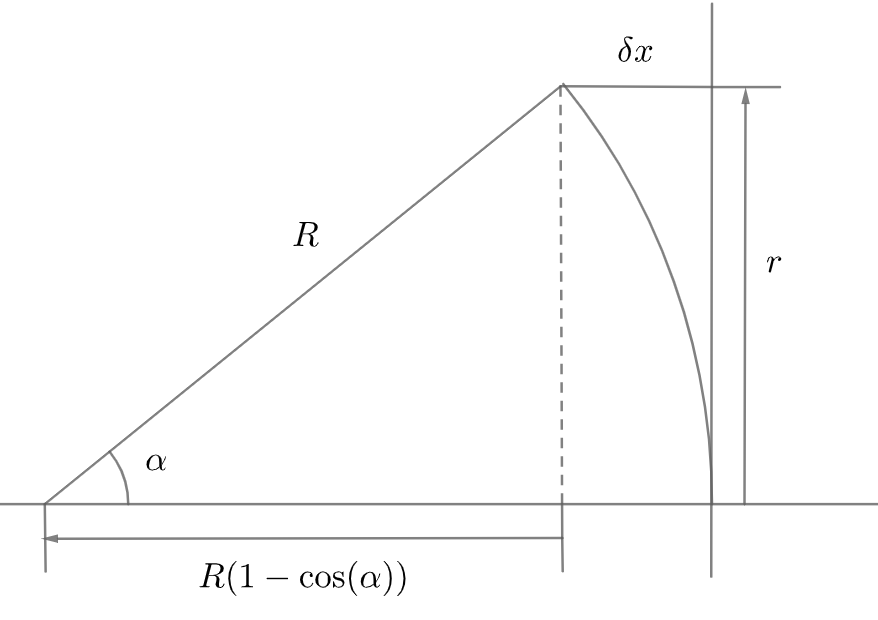
\includegraphics[width=0.6\textwidth]{drawing-for-phi}%
  \caption{A drawing showing how to compute \(\phi(r)\)}\label{fig:phi-of-r}%
\end{figure}
We can conclude now that

\begin{equation}
  \left( \frac{1}{q} \right)_r = \frac{1}{R}\,.
\end{equation}

The imaginary part of \(\frac{1}{q}\) appears in the real exponential. This exponential should thus give the Gaussian distribution form of the wave, that is it should look like

\begin{equation}
  \ee^{-\left( \frac{r}{r_0} \right)^2}\,,
\end{equation}
where \(r_0\) is proportional to the standard deviation. In this case we can write

\begin{equation}
  \left(\frac{1}{q}\right)_i = \frac{2}{k w^2 (z)} = \frac{\lambda}{\pi w^2 (z)}\,.
\end{equation}
This defines the \textit{beam radius} \(w(z)\) as the value of \(r\) at which the field falls to \(\frac{1}{\ee}\) of its value on the z-axis. Putting these results together, we reach a final formula for \(\frac{1}{q}\)

\begin{equation}
  \label{sol:1-over-q}
  \frac{1}{q} = \frac{1}{R(z)} - \ii \frac{\lambda}{\pi w^2 (z)}\,.
\end{equation}

It is conventional to take \(\lim_{z\to0} R(z) \rightarrow \infty\), such that \(\frac{1}{q(0)} = -\ii \frac{\lambda}{\pi w_0^2}\), and \(w_0=w(0)\) is usually interpreted as the \textit{beam waist radius}. If we look back at the solution~(\ref{sol:q}), we can rewrite \(q\) in this formalism as

\begin{equation}
  \label{sol:q-better}
  q = z + \ii \frac{\pi w_0^2}{\lambda}\,.
\end{equation}
Playing around with~\cref{sol:1-over-q,sol:q-better} we have the following developement

\begin{equation*}
  \frac{1}{q} = \frac{1}{R} - \ii \frac{\lambda}{\pi w^2} = \frac{1}{z+ \ii \frac{\pi w_0}{\lambda}} = \frac{z - \ii \frac{\pi w_0}{\lambda}}{z^2 + \left(\frac{\pi w_0^2}{\lambda} \right)^2}
\end{equation*}

\begin{equation*}
  \frac{1}{R} = \frac{z}{z^2 + \left(\frac{\pi w_0^2}{\lambda} \right)^2} \Rightarrow R = z + \frac{1}{z} \left(\frac{\pi w_0^2}{\lambda} \right)^2
\end{equation*}

\begin{equation*}
  \frac{1}{w^2} = \frac{\frac{\pi^2 w_0^2}{\lambda^2}}{z^2 + \left(\frac{\pi w_0^2}{\lambda} \right)^2} \Rightarrow w = w_0 \sqrt{1+ \left(\frac{\lambda z}{\pi w_0^2}\right)^2}\,.
\end{equation*}

For the sake of clarity, I write again the expressions obtained for the radius of curvature and the beam radius

\begin{equation}
  R = z + \frac{1}{z} \left(\frac{\pi w_0^2}{\lambda} \right)^2
\end{equation}

\begin{equation}
  w = w_0 \sqrt{1+ \left(\frac{\lambda z}{\pi w_0^2}\right)^2}\,.
\end{equation}

Turning back now to~\cref{eq:G}, using~(\ref{sol:q-better}), we can rewrite it as

\begin{equation*}
  \frac{\dd{G}}{G} = - \frac{\dd(z+\ii \frac{\pi w_0^2}{\lambda})}{z + \ii \frac{\pi w_0^2}{\lambda}}\,,
\end{equation*}
which, after integration, becomes

\begin{equation*}
  \ln{\frac{G(z)}{G(0)}} = \ln{\frac{z+\ii \frac{\pi w_0^2}{\lambda}}{\ii \frac{\pi w_0^2}{\lambda}}}
\end{equation*}
or

\begin{equation}
  \frac{G(z)}{G(0)} = \frac{1}{1 - \ii \frac{\lambda z}{\pi w_0^2}} = \frac{1 + \ii \frac{\lambda z}{\pi w_0^2}}{1 +\left(\frac{\lambda z}{\pi w_0^2}\right)^2}\,.
\end{equation}
For convenience, this is usually expressed interms of a phasor (commonly called Gouy phase) defined as

\begin{equation}
  \tan(\phi_0) = \frac{\lambda z}{\pi w_0^2}\,.
\end{equation}
Now the solution for \(G\) is stylized to be

\begin{equation}
  \label{sol:G}
  \frac{G(z)}{G(0)} = \frac{w_0}{w} \ee^{\ii \phi_0}\,.
\end{equation}
Putting together~\cref{def:guess-gauss,sol:1-over-q,sol:G} we finally find \(u\)

\begin{equation}
  u(r,z) = G(0) \frac{w_0}{w} \exp(-\frac{r^2}{w^2} - \ii \frac{\pi r^2}{\lambda R} + \ii \phi_0)
\end{equation}
and, consequently, the solution to the paraxial wave equation with axial symmetry

\begin{equation}
  \label{sol:final}
  \zeta(r,z) = G(0)\frac{w_0}{w} \exp(-\frac{r^2}{w^2}  -\ii k z -\ii \frac{\pi r^2}{\lambda R} + \ii \phi_0)\,.
\end{equation}

\subsection{Gaussian Beam Packets}

In the reaserch literature, it is a custom to use a parameter called \textit{confocal distance} or \textit{Reyleigh range}

\begin{equation}
  z_0=\frac{\pi w_0^2}{\lambda} \,.
\end{equation}
Including it, all the relevant auxiliary functions become

\begin{subequations}
  \begin{align}
    R(z) = z+\frac{z_0^2}{z} \\
    w(z) = w_0 \sqrt{1+\left( \frac{z}{z_0}\right)^2}\\
    \phi_0 (z) = \arctan(\frac{z}{z_0}) \,.
  \end{align}
\end{subequations}

We can immediately observe that \(w(z)\) at \(z=z_0\) is actually equal to \(\sqrt{2}w_0\). From this we can deduce that the \(z_0\) indicates how far from the origin the beam is collimated. It is very simple to understand by looking at figure~\cref{fig:gauss-beam}

\begin{figure}[h]
  \centering
  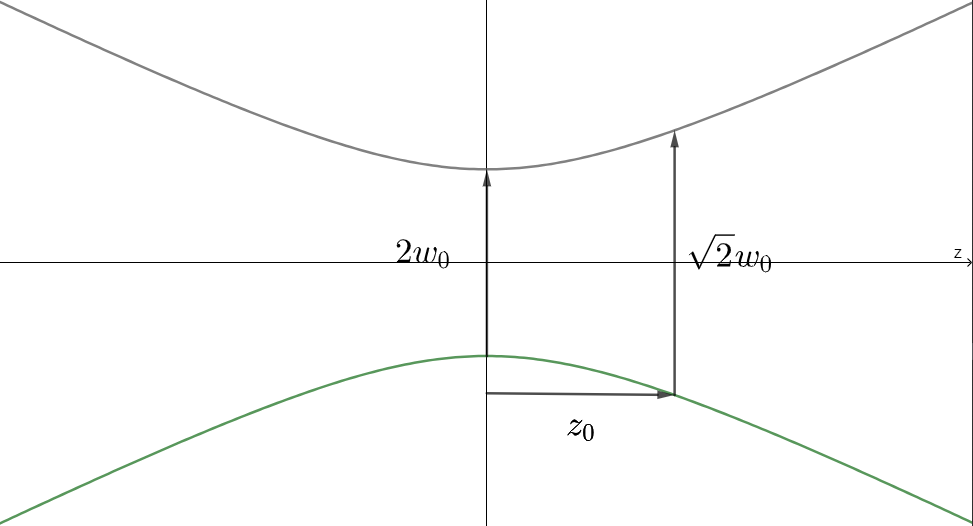
\includegraphics[width=0.9\textwidth]{Gauss-beam-profile}%
  \caption{Gaussian beam radius \(w\) as a function of \(z\)}\label{fig:gauss-beam}%
\end{figure}

We can also differentiate three cases of interest for the curvature radius \(R(z)\). At \(z\rightarrow 0\), \textit{i}.\textit{e}. near the waist, \(R\rightarrow\infty\), so the profile is that of a plane wave. At the Reyleigh range, the curvature (\(\frac{1}{R}\)) is maximum and, consequently, the radius itself is minimum (\(2z_0\)). Finally, at very large distances away from the waist, the radius is equal to \(z\), so the profile is spherical.

The Gouy phase is an important parameter in theoretical considerations, especially when it comes to higher order Gaussian modes, but is hard to observe experimentally. Physically, it modifies the wavelength near the waist~(\cite{paschottaArticleGouyPhase}). This results also in a change of the phase velocity. As a consequence, the phase velocity near the waist can exceed the velocity of light in the medium, just as it might inside a waveguide.

Now that we understood the shape and behaviour of the Gauss beam, we are almost ready to define the electric and magnetic fields. But before that we must talk about normalization. While a look at~(\ref{sol:final}) might not suggest the need for any normalization, physical arguments request it. We would like to not have unexplained losses of power as a funtion of \(z\) (remember that we are basically just setting the dependence of the fields on position right now). As such, a normalization of \(\zeta(r,z)\) over the transversal surface is necessary. That is, we want the intensity as a function of \(z\) to be just a constant. While in literature is very common to impose norm 1, I find it more useful to norm it to \(\pi w_0^2\), as suggested by~\cite{donderaElectronsTwistedFields2020}, such that the final result is adimensional and it is easier to introduce the amplitude of the field. We have

\begin{equation*}
  \pi w_0^2 = \iint \dd{r}\dd{\varphi} r\abs{\zeta}^2 = 2 \pi \abs{G(0)}^2 \int \dd{r} \abs{\frac{w_0}{w}}^2 r \ee^{-2\frac{r^2}{w^2}} =
\end{equation*}

\begin{equation*}
  = \frac{1}{2}\pi \left(\frac{w_0}{w}\right)^2 \abs{G(0)}^2 w^2\int \dd{\left(2\frac{r^2}{w^2}\right)} \ee^{-2\frac{r^2}{w^2}} =
\end{equation*}

\begin{equation*}
  = \frac{1}{2}\pi w_0^2 G^2(0)
\end{equation*}
which gives the normalization constant

\begin{equation}
  G(0) = \sqrt{2}\,.
\end{equation}

\subsubsection{The Electric Field}
The \(x\) and \(y\) components of the electric field are now expressed using~\cref{sol:final} as

\begin{subequations}
  \label{def:gauss-beam-fields-xy}
  \begin{align}
    E_x (r,z) = \alpha_x E_0 \sqrt{2}\frac{w_0}{w} \exp(-\frac{r^2}{w^2}  -\ii k z -\ii \frac{k r^2}{2 R} + \ii \phi_0)\\
    E_y (r,z) = \alpha_y E_0 \sqrt{2}\frac{w_0}{w} \exp(-\frac{r^2}{w^2}  -\ii k z -\ii \frac{k r^2}{2 R} + \ii \phi_0)\,,
  \end{align}
\end{subequations}
where we choose \(\alpha_x=1\), \(\alpha_y=0\) for linear polarization, and \(\alpha_x=\frac{1}{\sqrt{2}}\), \(\alpha_y=\pm \frac{\ii}{\sqrt{2}}\) for right and left-handed circular polarization, respectively. In order to obtain the \(z\) component, we have to impose the condition \(\div{\vb{E}} = 0\) and to use the approximation \(\partial_z E_z \approx -\ii k E_z\) (which holds if the pulse is long enough or quasi-rectangular). The immediate result is

\begin{equation}
  E_z (r,z) = - \frac{\ii}{k} \left( \partial_x E_x (r,z) +\partial_y E_y (r,z)\right)\,,
\end{equation}
or, explicitly

\begin{equation}
  E_z (r,z) = \frac{2 \left(\ii -\frac{z}{z_0}\right)}{kw^2 (z)} [xE_x (r,z) +yE_y(r,z)]\,.
\end{equation}

\subsubsection{The Magnetic Field}
In order to derive the magnetic, one can impose the relation~(\ref{othogonality-of-fields})

\begin{equation*}
  \vb{B} = \frac{1}{c} \vb{n} \cp\vb{E} = \frac{1}{c} \vb{e_z} \cp\vb{E} = \frac{1}{c} E_x \vb{e_z} \cp\vb{e_x} + \frac{1}{c} E_y \vb{e_z} \cp\vb{e_y} = - \frac{1}{c} E_y \vb{e_x}+\frac{1}{c} E_x \vb{e_y} \,,
\end{equation*}
which indicates that

\begin{subequations}
  \begin{align}
    B_x(r,z) = -\frac{1}{c}E_y(r,z)\\
    B_y(r,z) = \frac{1}{c}E_x(r,z)\,.
  \end{align}
\end{subequations}
The third component is found exactly in the same way as for the electric field, taking into account that \(\div{\vb{B}}=0\) and using the same approximation \(\partial_z B_z \approx -\ii k B_z\) (the conditions for its validity are the same):

\begin{equation}
  B_z (r,z) = - \frac{\ii}{k} \left( \partial_x B_x (r,z) +\partial_y B_y (r,z)\right) = -\frac{\ii}{ck} \left( \partial_y E_x (r,z) - \partial_x E_y (r,z) \right)\,,
\end{equation}
or rather

\begin{equation}
  B_z (r,z) = \frac{2 \left(\ii -\frac{z}{z_0}\right)}{ckw^2 (z)} [yE_x (r,z) -xE_y(r,z)]\,.
\end{equation}

\subsubsection{The Temporal Profile}
One observation must be made now. These expressions only describe the spatial part of the field. In order to give the exact field we must add the time-dependent part of the solution \(\ee^{\ii \omega t}\). However, this is not all there is to it. Since we are interested in describing laser beams, we must take into consideration the fact that the pulse has a finite duration. One does this by adding a Gaussian envelope over time. The time-dependent part will now be

\begin{equation}
  \label{temporal-profile}
  g(z,t) = \exp(\ii \omega t - \left( \frac{t-\frac{z-z_F}{c}}{\tau_0}\right)^2)\,,
\end{equation}
where \(\tau_0\) is the duration of the pulse and \(z_F\) is the original position of the intensity peak.

In what follows, I aim to provide a short proof of the fact that even with this envelope, the final fields are still solutions of Helmholtz equation under the paraxial approximation.

Let \(f(r,z)\) be the solution for

\begin{equation}
  \partial_r^2 f +\frac{1}{r} \partial_r f - 2\ii k \partial_z f = 0\,.
\end{equation}
The solution for the complete Helmholtz equation

\begin{equation}
  \partial_r^2 u +\frac{1}{r} \partial_r u +\partial_z^2 u -\frac{1}{c} \partial_t^2 u = 0
\end{equation}
is proposed to be \(u(r,z) = f(r,z) g(z,t) \ee^{-\ii k z}\) such that we have

\begin{equation*}
  \partial_r^2 (fg\ee^{-\ii k z}) +\frac{1}{r} \partial_r (fg\ee^{-\ii k z}) +\partial_z^2 (fg\ee^{-\ii k z}) -\frac{1}{c^2} \partial_t^2 (fg\ee^{-\ii k z}) = 0
\end{equation*}

\begin{equation*}
  (\partial_r^2 f +\frac{1}{r} \partial_r f) g\ee^{-\ii k z} + (\partial_z^2 f) g\ee^{-\ii k z} + 2 (\partial_z f) \partial_z (g\ee^{-\ii k z}) + f \partial_z^2(g\ee^{-\ii k z}) - \frac{1}{c^2} f \partial_t^2 (g\ee^{-\ii k z}) = 0\,.
\end{equation*}
The paraxial approximation allows us to ignore the \(\partial_z^2 f\) term
\begin{equation*}
  (\partial_r^2 f +\frac{1}{r} \partial_r f) g\ee^{-\ii k z} + 2 (\partial_z f) \partial_z (g\ee^{-\ii k z}) + f \partial_z^2(g\ee^{-\ii k z}) - \frac{1}{c^2} f \partial_t^2 (g\ee^{-\ii k z}) = 0
\end{equation*}

\begin{equation*}
  (\partial_r^2 f +\frac{1}{r} \partial_r f - 2 \ii k \partial_z f) g\ee^{-\ii k z} + 2 (\partial_z f) \ee^{-\ii k z} \partial_z g+ f \partial_z^2(g\ee^{-\ii k z}) - \frac{1}{c^2} f \partial_t^2 (g\ee^{-\ii k z}) = 0
\end{equation*}

\begin{equation*}
  (\partial_r^2 f +\frac{1}{r} \partial_r f - 2 \ii k \partial_z f) g\ee^{-\ii k z} +f \left[ 2 \frac{\partial_z f}{f} \ee^{-\ii k z} \partial_z g+ \partial_z^2(g\ee^{-\ii k z}) - \frac{1}{c^2} \partial_t^2 (g\ee^{-\ii k z}) \right] = 0\,.
\end{equation*}

The first term is zero since \(f\) is a solution, so we must have the second term also equal to zero

\begin{equation*}
  2 \frac{\partial_z f}{f} \ee^{-\ii k z} \partial_z g+ \partial_z^2(g\ee^{-\ii k z}) - \frac{1}{c^2} \partial_t^2 (g\ee^{-\ii k z})= 0
\end{equation*}

\begin{equation*}
  2 \frac{\partial_z f}{f} \ee^{-\ii k z} \partial_z g+ (\partial_z^2g)\ee^{-\ii k z} -2\ii k (\partial_z g) \ee^{-\ii k z} - k^2 g \ee^{-\ii k z} - \frac{1}{c^2} (\partial_t^2 g)\ee^{-\ii k z}= 0
\end{equation*}
and eliminating the exponential

\begin{equation*}
  2 \frac{\partial_z f}{f} \partial_z g+ \partial_z^2 g -2\ii k \partial_z g- k^2 g- \frac{1}{c^2} \partial_t^2 g= 0
\end{equation*}
or, using \(ck=\omega\)

\begin{equation}
  2 \ii \omega c \partial_z g +\partial_t^2 g + \omega^2 g=c^2 \partial_z^2 g + 2 c^2 \frac{\partial_z f}{f} \partial_z g\,.
\end{equation}
Based on~\cref{temporal-profile} we have

\begin{equation}
  \partial_z g = \frac{2}{c} \frac{t-\frac{z-z_F}{c}}{\tau_0^2} g \Rightarrow 2 \ii \omega c \partial_z g = 4\ii \omega \frac{t-\frac{z-z_F}{c}}{\tau_0^2} g
\end{equation}

\begin{equation}
  \partial_z^2 g = - \frac{2}{c^2} \frac{1}{\tau_0^2} g + \frac{4}{c^2} \left(\frac{t-\frac{z-z_F}{c}}{\tau_0^2} \right)^2 g \Rightarrow c^2\partial_z^2 g = - 2 \frac{1}{\tau_0^2} g+ 4 \left(\frac{t-\frac{z-z_F}{c}}{\tau_0^2} \right)^2 g
\end{equation}

\begin{equation}
  \partial_t g = \left(\ii \omega - 2 \frac{t-\frac{z-z_F}{c}}{\tau_0^2} \right) g
\end{equation}

\begin{equation}
  \partial_t^2 g = - 2 \frac{1}{\tau_0^2} g + \left(\ii \omega - 2 \frac{t-\frac{z-z_F}{c}}{\tau_0^2} \right)^2 g = - 4\ii \omega \frac{t-\frac{z-z_F}{c}}{\tau_0^2} g - 2 \frac{1}{\tau_0^2} g - \omega^2 g+ 4 \left(\frac{t-\frac{z-z_F}{c}}{\tau_0^2} \right)^2 g
\end{equation}
Summing everything up, we still remain with a

\begin{equation}
  \frac{\partial_z f}{f} \partial_z g = 0\,,
\end{equation}
which is true under the paraxial approximation. %why?

It is important to mention that this profile is not always usable. According to~\cite{quesnelTheorySimulationInteraction1998} finite pulse effects are important for \(c\tau_0  \lessapprox 2w_0\), and in this situation we must put an additional \(2 \partial_z
 g \partial_z \vb{E}\) in the paraxial wave equation.

\subsubsection{The Final Fields}

The final relations are straightforward

\begin{subequations}
  \begin{align}
    \vb{E}(r,z,t) = \vb{E}(r,z) g(t,z) \\
    \vb{B}(r,z,t) = \vb{B}(r,z) g(t,z)\,.
  \end{align}
\end{subequations}

\subsection{Laguerre-Gauss Beams}
This tipe of beam represents a correction for the Gauss one in order to remove the axial symmetry approximation. That is, we want fo find a function \(f(r,z,\varphi) = \zeta (r,z) s(r,z,\varphi)\) to be a solution of

\begin{equation}
  \partial_r^2 f +\frac{1}{r} \partial_r f + \frac{1}{r} \partial_\varphi^2 f - 2 \ii k \partial_z f = 0 \,,
\end{equation}
where \(\zeta\) is found in~(\ref{sol:final}). Actually, we would rather make an educated guess for a trial solution

\begin{equation}
  f(r,z,\varphi) = \zeta (r,z) S(r) \ee^{im\varphi}\,,
\end{equation}
with \(m\) can be a real number. In this case, it is straightforward to find that \(S(r)\) turns out to satisfy an equation similar to that of the associated Laguerre polynomials. One can reach through not so short computations the expression

\begin{equation}
  S(r) = \left(\frac{\sqrt{2r}}{w(z)}\right)^m L_{pm}\left(\frac{2r^2}{w^2(z)}\right)\,.
\end{equation}

The associated (or sometimes also called generalized) Laguerre polynomials are a solution of~(\cite{abramowitzHandbookMathematicalFunctions2013})

\begin{equation}
  x L_{pm}''(x) + (m+1-x) L_{pm}'(x) + p L_{pm}(x) =0\,,
\end{equation}
where \(p\in\mathbb{N}\) and \(m\in\mathbb{R}\).
Their expression can be obtained using the Rodrigues formula

\begin{equation}
  L_{pm} (x) = \frac{x^{-m} e^x}{p!} \dv[p]{x} (e^{-x} x^{m+p})\,.
\end{equation}

We will now apply the same normalization criterion we used for the Gauss mode for \(f(r,z,\varphi)\)

\begin{equation}
  \pi w_0^2 = \iint \dd{r}\dd{\varphi} r \abs{f}^2\,.
\end{equation}
The integration is done as such

\begin{equation*}
  do\; it\; already
\end{equation*}

The final expressions for the electric field, after dealing with normalization, are

\begin{subequations}
  \begin{align}
    E_x^{pm} (r,z,\varphi) = E_x(r,z) \sqrt{\frac{p!}{(\abs{m}+p)!}} \left(\frac{\sqrt{2}r}{w(z)}\right)^{\abs{m}} L_{p\abs{m}} \left(\frac{2r^2}{w^2(z)}\right) \exp(\ii (2p+\abs{m}) \arctan(\frac{z}{z_0}))\ee^{-\ii m \varphi} \\
    E_y^{pm} (r,z,\varphi) = E_y(r,z) \sqrt{\frac{p!}{(\abs{m}+p)!}} \left(\frac{\sqrt{2}r}{w(z)}\right)^{\abs{m}} L_{p\abs{m}} \left(\frac{2r^2}{w^2(z)}\right) \exp(\ii (2p+\abs{m}) \arctan(\frac{z}{z_0}))\ee^{-\ii m \varphi} \\
    E_z^{pm} (r,z,\varphi) = - \frac{i}{k} \left(\partial_x E_x^{pm} (r,z,\varphi) + \partial_y E_y^{pm} (r,z,\varphi) \right) \,,
  \end{align}
\end{subequations}
where \(E_x(r,z)\) and \(E_y(r,z)\) are to be taken from the Gaussian beam~(\ref{def:gauss-beam-fields-xy}). For the sake of use in numerical simulations (mainly to eliminate the need for numerical differentiation) the \(z\) component of the field can be computed explicitly to be

\begin{equation}
  \begin{aligned}
    E_z^{pm} = - \frac{\ii}{k} \left(-2\frac{1+\ii\frac{z}{z_0}}{w^2(z)} +\frac{L_{p\abs{m}}'\left(\frac{2r^2}{w^2(z)}\right)}{L_{p\abs{m}}\left(\frac{2r^2}{w^2(z)}\right)}\right) \left( xE_x^{pm} + yE_y^{pm} \right) - \\
    -\frac{\ii}{k}\sqrt{\frac{p!}{(\abs{m}+p)!}} \left(\frac{\sqrt{2}}{w(z)}\right)^{\abs{m}} L_{p\abs{m}} \left(\frac{2r^2}{w^2(z)}\right) \exp(\ii (2p+\abs{m}) \arctan(\frac{z}{z_0})) (A_x E_x + A_y E_y)\,,
  \end{aligned}
\end{equation}
with

\begin{subequations}
  \begin{align}
    A_x =
    \begin{cases}
      l (x - \ii y)^{l-1} , \; l>0 \\
      0,\;l=0\\
      -l(x+\ii y)^{-l-1},\; l<0
    \end{cases} \\
    A_y =
    \begin{cases}
      -\ii l (x - \ii y)^{l-1} , \; l>0 \\
      0,\;l=0\\
      -\ii l(x+\ii y)^{-l-1},\; l<0\,.
    \end{cases}
  \end{align}
\end{subequations}
The magnetic field is derived exactly as in the case of the Gaussian beam

\begin{subequations}
  \begin{align}
    B_x(r,z,\varphi) = -\frac{1}{c}E_y(r,z,\varphi)\\
    B_y(r,z,\varphi) = \frac{1}{c}E_x(r,z,\varphi)\\
    B_z (r,z,\varphi) = -\frac{\ii}{ck} \left[ \partial_y E_x (r,z,\varphi) - \partial_x E_y (r,z,\varphi) \right] \,.
  \end{align}
\end{subequations}
The explicit third component of \(\vb{B}\) is

\begin{equation}
  \begin{aligned}
  B_z^{pm} = - \frac{\ii}{ck} \left(-2\frac{1+\ii\frac{z}{z_0}}{w^2(z)} +\frac{L_{p\abs{m}}'\left(\frac{2r^2}{w^2(z)}\right)}{L_{p\abs{m}}\left(\frac{2r^2}{w^2(z)}\right)}\right) \left( yE_x^{pm} - xE_y^{pm} \right) - \\
  -\frac{\ii}{ck}\sqrt{\frac{p!}{(\abs{m}+p)!}} \left(\frac{\sqrt{2}}{w(z)}\right)^{\abs{m}} L_{p\abs{m}} \left(\frac{2r^2}{w^2(z)}\right) \exp(\ii (2p+\abs{m}) \arctan(\frac{z}{z_0})) (A_y E_x - A_x E_y)\,.
  \end{aligned}
\end{equation}
These expressions are easier to derive if we bring together the terms \(\left(\frac{\sqrt{2}r}{w(z)}\right)^{\abs{m}}\) and \(\ee^{-\ii m \varphi}\) and replace \(r\ee^{\pm\ii \varphi}\) with \(x\pm\ii y\) before computing the derivatives. This step also helps to eliminate the apparent singularity that might appear on the z-axis. Also, it might be useful to write the derrivative of the associated Laguerre polynomial as

\begin{equation}
  L_{p\abs{m}}'\left(\frac{2r^2}{w^2(z)}\right) =
  \begin{cases}
    - \frac{4}{w^2(z)} L_{p-1,\abs{m}+1}'\left(\frac{2r^2}{w^2(z)}\right),\; 1\leq p\\
    0,\; otherwise\,.
  \end{cases}
\end{equation}

Of course, in order to use these relations in simulations involving laser beams, one must attach also the temporal profile~(\ref{temporal-profile}).

\subsection{Other Types of Gauss Beams}

One can only work in Carthesian coordinates in order to solve the paraxial wave equation. This will lead to obtaining the rectangular Gauss beam mode. The extension of this solution, in the same manner used to extend the cylindrical mode to the Laguerre-Gauss mode, is the Hermite-Gauss beam and, as the name suggests, uses the Hermite polynomials. However, these modes are not of interest in our endeavours. If the reader is interested to look upon them, the book by~\cite{goldsmithQuasiopticalSystemsGaussian1998} has a very concise and straightforward presentation of them in its first chapter.

\subsection{Bessel Beams}
%I wish:)
\section{Angular Momentum of Electromagnetic Waves}

\end{document}
